\section{Results Comparison and Analysis}
\label{cha:results}

In previous chapters, four algorithms to optimize 0--1 loss function have been proposed and analyzed. Two of them, the final branch and bound (BnB -- Algorithm \ref{alg:BnB.Final}) and the prioritized combinatorial search (PCS -- Algorithm \ref{alg:cs.prioritized}), can guarantee that the returned solution is optimal. The other two, combinatorial search approximation (CSA -- Algorithm \ref{alg:cs.approximation}) and smooth loss approximation (SLA -- Algorithm \ref{alg:sla.algorithm}), are approximation algorithms, and hence do not guarantee the optimality of the returned solution. However, these approximation algorithms are much more efficient, while their results have been shown to be quite close to the optimal solutions. All algorithms are designed as anytime algorithm, so that they can provide good solution even if terminated early. This chapter concentrates on providing a comprehensive comparison of these algorithms. To be more specific, the first section herein describes the testing platform and some common procedures for tests given in this chapter (and also for all tests conducted so far). The second section compares 0--1 loss optimization algorithms with each other, and  the third section compares them with other existing commonly used and state-of-the-art methods. Finally, the last section summarizes all interesting results of this chapter.


%=================================================
\subsection{Common Testing Platform and Procedures}
\label{sec:rc.method}

Common platform and procedures for all tests in this thesis are as follows. 

%======================
\subsubsection{Testing Platform}

All tests in this thesis are implemented in MATLAB 7.12.0 running in a Windows XP virtual machine with dual-core, 1GB RAM. The Windows XP OS is virtualized by VMWare Fusion, which in turn runs on a notebook operated by MacOS X Lion with 1.7GHz dual-core i5 Intel processor and 4GB RAM. 

%======================
\subsubsection{Softwares for Comparing Algorithms}

Several commonly used existing algorithms are compared with proposed algorithms in this thesis. The softwares used for those comparing algorithms are as follows. Software for linear support vector machines and logistic regression is by \cite{linearSVM}, with software available at \url{http://www.csie.ntu.edu.tw/~cjlin/liblinear}. Software for Bayes point machine is by \cite{bpm}, and is available at \url{http://research.microsoft.com/en-us/um/people/minka/papers/ep/bpm}.

%======================
\subsubsection{Results Comparison Method}

If not otherwise mentioned, comparison of results and statement of improvement are based on the paired Student's t-test at $\alpha = 0.05$.  

%======================
\subsubsection{Synthetic Datasets Generation}

Synthetic testing datasets are generated as follows: 
\begin{enumerate}
  \setlength{\itemsep}{4pt}
  \setlength{\parskip}{1pt}
  \setlength{\parsep}{1pt}
	\item A common data range $R$ is randomly select between 5 and 10. 
	\item Two center points $C_1, C_2$, each corresponding to one class, are randomly chosen in the range $\pm (R/2)$ from the origin. 
	\item Variances in every dimension of the two center points $C_1, C_2$ are specified randomly in range $[1, R^2]$. 
	\item The desired number of data points for each class are then generated by a normal distribution with mean at $C_1$ or $C_2$ respectively, and a covariance matrix having corresponding variances on the main diagonal and 0 elsewhere.     
	\item If a specific range of 0--1 loss value is required. The dataset is repeatedly generated by the above step, and then checked by PCS algorithm until its 0--1 loss value is within the desired range.
\end{enumerate}

%======================
\subsubsection{Real-World Datasets for Testing}

Some tests use real-world datasets, which are taken from the UCI machine learning repository by \cite{ucidata}. These datasets are listed in Table \ref{tab:datasets}.

\begin{table*}[htbp!]
\centering
\begin{tabular}{c  c c l}
\hline\hline
Dataset & $N$ & $D$ & Name \& Source \\
\hline
Breast & 683 & 10 & Breast Cancer, \cite{breast} \\
Liver & 345 & 6 & Liver Disorders, UCI \\
Cmc & 1473 & 9 & Contraceptive Method Choice, UCI\\
Heart & 270 & 13 & Statlog (Heart), UCI\\
Indian & 583 & 10 & Indian Liver Patient, UCI\\
Pima & 768 & 8 & Pima Indians Diabetes, UCI\\
Sonar & 208 & 60 & Connectionist Bench (Sonar, Mines vs. Rocks), UCI\\
\hline\hline
\end{tabular}
\caption{Size, name, and source of real-world testing datasets.} 
\label{tab:datasets}
\end{table*}

%======================
\subsubsection{Data Preprocessing and Noise Generation}
The following are common procedures for data preprocessing and noise generation:
\begin{itemize}
\item \emph{Data preprocessing:} if not otherwise stated, all testing datasets use standardized features (data are normalized features-wisely to have mean-0 variance-1 before being passed as an input to any algorithm). 
\item \emph{Noise:} If it is mentioned that a certain percentage of noise is added to the dataset, then this step is done prior to data preprocessing. Noise is generated randomly and uniformly in the range from $min - 0.5(max-min)$ to $max + 0.5(max-min)$ of each dimension of the dataset, where $min, max$ are minimum and maximum value of data in the given dimension. Noise is then assigned to the first class of the dataset. Because the range of noise is twice the range of data, this process produces both background noise and outliers.
\end{itemize}


%=================================================
\subsection{Comparison Between Proposed Algorithms}
\label{sec:rc.proposed}

In this section, the four algorithms proposed in this thesis are being compared between themselves. As stated above, these algorithms can be divided into two categories: algorithms guaranteeing optimality, and approximation algorithms. Clearly, the first category of algorithms have higher complexity, therefore they are suitable for smaller datasets. On the other hand, the algorithms in the second category have much lower complexity and they can handle bigger datasets. It is, thus, natural to structure the comparison in this section in accordance with the these two categories, as follows.    

%=========================
\subsubsection{Correctness of Algorithms Guaranteeing Optimality}
\label{ssec:rc.optimal}

The BnB and PCS algorithms are compared with each other in this subsection. Since both these algorithms guarantee the optimality of the returned results, the goal of the test here is the verification of this fact. 1000 synthetical testing datasets have been generated with different size $N \in [20, 35]$, dimensionality $D \in [2, 4]$, and minimum loss $\in [0, 10]$. Each dataset is tested with each of the two algorithms, and the results show that for 74 of 1000 cases, the 0--1 loss returned by PCS is by 1 unit greater than that of BnB, and for the remaining cases their results coincide. The correlation coefficient of PCS and BnB is 0.9795, while we note that the 74 odd cases were likely caused by limited numerical precision of Matlab. Considering the fact, that these two algorithms are from unrelated approaches, so if one or both of them are incorrect (i.e. not guaranteeing optimality), their returned 0--1 loss would likely differ much more. The fact that their results are almost identical convinces that both algorithms return optimal solutions. 

In the test described above, the running times of each algorithm have been also recorded. The results show that the average running time of the BnB algorithm is 2.04 seconds with standard deviation 5.38, while these numbers are 0.16 and 0.17 for the PCS algorithm. Clearly, PCS offers lower and more stable running times than the BnB for the generated low dimensionality datasets. Thus, PCS is used in the remaining parts of this chapter whenever references to optimal 0--1 loss solutions are required. However, this poses a question of interest: How would these algorithms perform with increasing dimensionality? This shall be answered in the next subsection. 

%=========================
\subsubsection{Running Time of Algorithms Guaranteeing Optimality}

\begin{figure}[here]
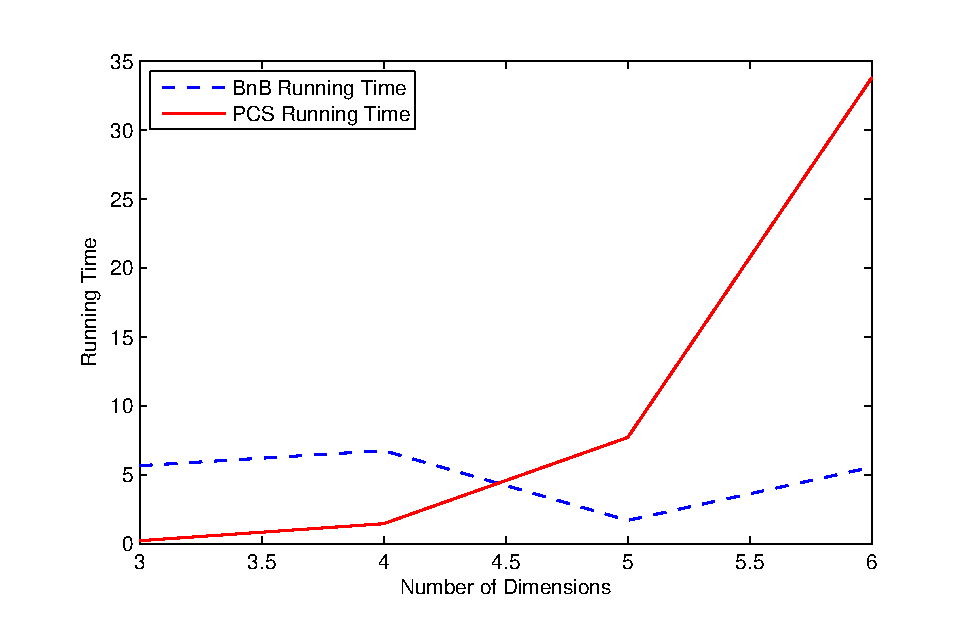
\includegraphics[width=0.50\textwidth]{images/fig62_622b.eps}
\caption{
This plot compares the running time of BnB and PCS algorithms with increasing dimensionality. Results are average over 20 restarts for each value of dimensionality $D$ from 3 to 6. As can be seen, the running time of PCS increases steadily with increasing number of dimensions, whereas BnB shows no dependence on dimensionality in this test. 
}
\label{fig:622a}
\end{figure}

To answer the question posed in the previous subsection on the dependence BnB and PCS on dimensionality, a test consists of synthetic datasets of size $N=30$ was conducted as follows. For each value of dimensionality $D$ from 3 to 6, twenty datasets were generated and tested on BnB and PCS. Figure \ref{fig:622a} shows the average running time corresponding to each value of $D$. It can be seen, that PCS strongly increases with dimensionality, while BnB doesn't seem so. It was, however, noted during the test, that BnB's running time is strongly dependent on the value of optimal 0--1 loss. This is expected, as higher optimal 0--1 loss value worsens the effectiveness of the bound of BnB, hence enlarges the search space exponentially. 

To sum up, for the case of exhaustive search to find the optimal solution, PCS running time increases rapidly with increasing dimensionality, while BnB running time increases with increasing optimal 0--1 loss value. In the next subsection, we shall examine how good these anytime algorithms work when being terminated early, i.e., in the role of approximation algorithms instead of those guaranteeing optimality.


%=========================
\subsubsection{Comparing Approximation Algorithms}
\label{ssec:rc.approx}

A detailed comparison between combinatorial search approximation (CSA) and adjustable loss approximation (SLA) has been made in Section \ref{sec:sla.algorithm} of Chapter \ref{cha:Smoothlossapprox}, especially through Figure \ref{fig:sla.approxsumm}, \ref{fig:sla.approxlosses}, and \ref{fig:sla.approxsumm2}. This comparison,  based on synthetic data, showed that the two approximation algorithms have very similar approximation accuracy, both near to the optimal solution, but SLA is by significantly more efficient. 

Thank to the anytime design, BnB and PCS can also be considered approximation algorithm if a running time threshold is specified. Therefore, they should also be compared with CSA and SLA. This comparison is performed on real-world datasets in Subsection \ref{ssec:rc.optimality2} together with several existing algorithms. Results of this comparison are shown in Tables \ref{tab:losses0noise} through \ref{tab:runningtimes}.


%=================================================
\subsection{Comparison with Other State-of-the-Art Methods}
\label{sec:rc.others}

Arguably, the most commonly used methods for binary linear classification are logistic regression (LR) and support vector machines (SVM). Beside those, Bayes point machines (BPM) is another state-of-the-art method, which is gaining popularity in binary classification. In this section, the novel algorithms shall be compared with these existing algorithms in different tests using both synthetic and real world datasets. The first two subsections here contain tests aiming at pointing out the differences in optimality of the returned solutions. It was mentioned at the beginning of the thesis that classification based on 0--1 loss is robust to outliers. Thus, the third subsection is devoted to comparing the prediction accuracy of the novel algorithms with existing algorithms in the presence of outliers. The last subsection examines a class of datasets termed anti-surrogate-loss, for which all algorithms based on surrogates to 0--1 loss give poor results, whereas novel algorithms work well. 


%=========================
\subsubsection{Optimality of Solutions on Synthetic Data}
\label{ssec:rc.optimality}

As discussed in Subsection \ref{ssec:rc.approx}, SLA is efficient and provide similar results comparing to other proposed algorithm. Thus, in this subsection, SLA is selected to represent all proposed algorithms in tests comparing the optimality of returned solutions with LR, SVM, and BPM. Two tests with synthetic datasets will be provided for the with and without noise scenarios. 

Note that for all tests conducted in this section, parameters for SLA algorithm are fixed at the values given by the example in Section \ref{sec:sla.algorithm}, and its initial approximation is given by the best solution of LR, which has linear running time and faster than SVM, hence more suitable. Parameters of existing algorithms are determined specifically for each dataset to give the best 0--1 loss.

\begin{figure}[ht!]
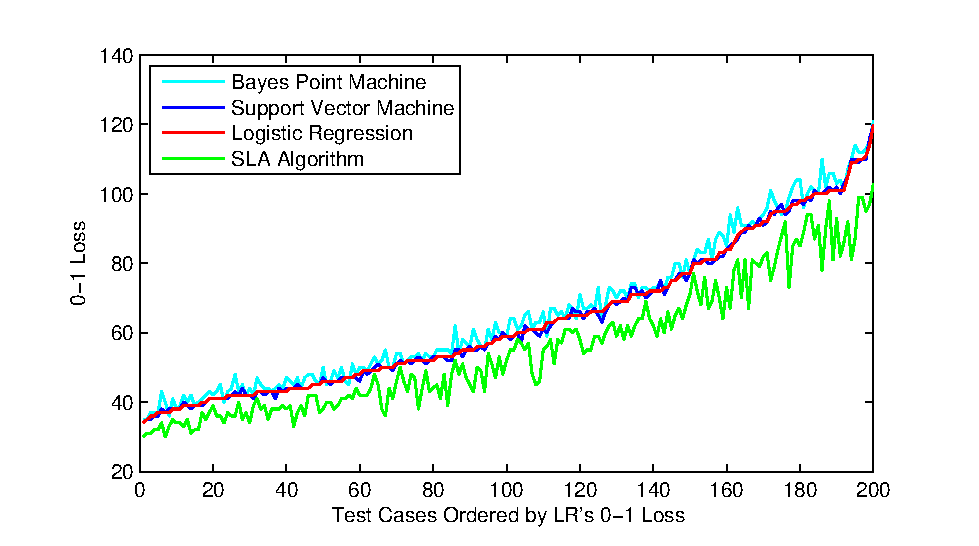
\includegraphics[width=0.50\textwidth]{images/fig61_621a.eps}
\caption{
This plot shows the 0--1 loss values by SLA algorithm comparing to other methods over 200 synthetic datasets of $N=500, D=5$ with optimal 0--1 loss in the range of $[30, 100]$. As can be seen, LR (red curve) seems to have a slightly lower loss than that of SVM, whereas BPM (cyan curve) tends to be higher in most of the cases. The 0--1 loss values returned by SLA (green curve) are significantly lower than that of all others, showing that SLA algorithm does very good job in optimizing 0--1 loss.  
}
\label{fig:621a}
\end{figure}

\begin{figure}[ht!]
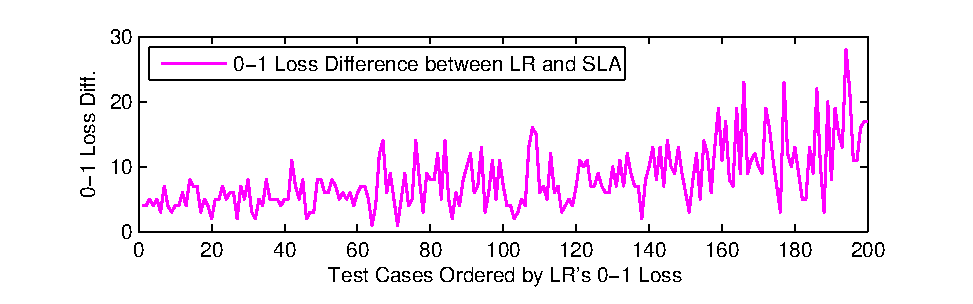
\includegraphics[width=0.50\textwidth]{images/fig61_621aDiff.eps}
\caption{
This plot shows the difference in 0--1 loss values between LR and SLA corresponding to the plot in Figure \ref{fig:621a}. The mean of the differences is 8.14 with standard deviation 4.72, representing about $12.8\% \pm 8.52\%$ of improvement of SLA over LR. The improvement is substantial with $p \ll 0.0001$ under t-test. 
}
\label{fig:621aDiff}
\end{figure}

\begin{figure}[here]
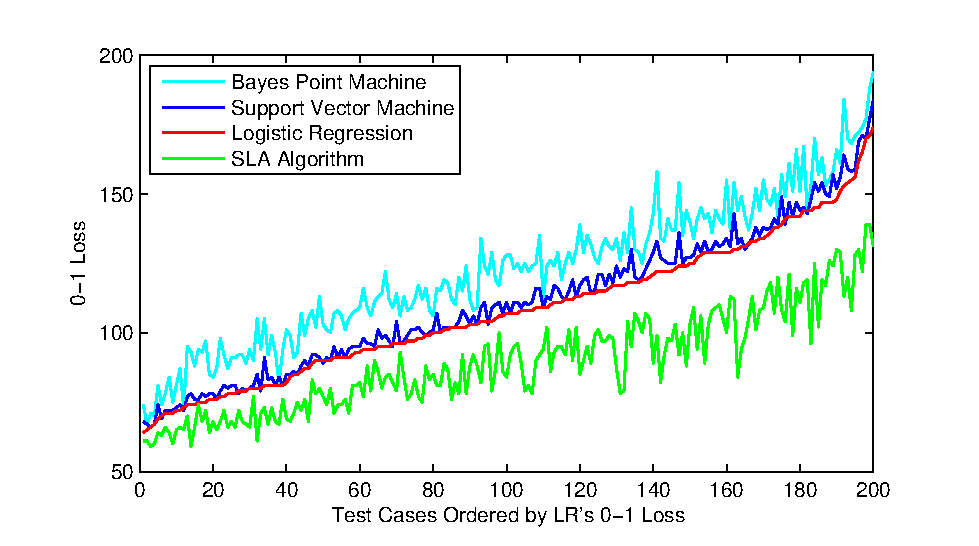
\includegraphics[width=0.50\textwidth]{images/fig61_621b.eps}
\caption{
This plot shows the 0--1 loss values returned by the comparing methods in presence of 15\% noise. The difference between SLA and other methods is more significant in this case. The SLA curve is positioned well below other curves and also increases at slower rate, and in some cases, SVM's loss is 45\% higher SLA's loss. Another notable differences is that BPM's losses are higher than SVM's, and LR has lower losses comparing to both SVM and BPM. 
}
\label{fig:621b}
\end{figure}

Firstly, to see the differences in returned 0--1 loss values of comparing algorithms. A test has been designed as follows. 200 datasets are generated with size $N=500$, dimensionality $D=5$, and optimal 0--1 loss in the range from 30 to 100. After preprocessing, these datasets are tested with each of the four methods and the 0--1 loss values of the solutions returned by each method are recorded. Figure \ref{fig:621a} shows the results of this test, where, for a better visualization, the results are ordered by increasing 0--1 loss values given by LR. As can be seen, SLA algorithm gives significantly lower 0--1 loss values than all other methods. In some cases, the loss value given by SVM can be more than 30\% higher than that given by SLA. Figure \ref{fig:621aDiff} concentrates on analysis of the differences between LR and SLA, where LR is chosen to represent SVM and BPM as it has similar or better results. It can be seen from this figure, that LR's 0--1 loss values are always higher than SLA's, and the level of difference is dataset specific (i.e. even for datasets with similar size, dimension, and optimal loss value, the differences fluctuate a lot). This suggests that there are datasets with some specific structure that is ``anti'' algorithms based on surrogate loss like LR, SVM, BPM. Subsection \ref{ssec:rc.anti} is devoted to examine these datasets. For the purpose here, the important message is that SLA shows a substantial improvement of $12.8\% \pm 8.52\%$ in 0--1 loss optimization in this test. The confidence of this improvement is supported by the t-test with $p \ll 0.0001$.

Secondly, to see how well different algorithms deal with noise and outliers, another test has been designed, in which datasets are generated the same way as in the previous test, except that 15\% of noise (including outliers) is added to every dataset, increasing its size to $N=575$. Figure \ref{fig:621b} visualizes the results of this test. The immediate thing to note in this figure is that the SLA curve is significantly lower than other curves, and it also increases at a slower rate. Clearly, the presence of noise and outliers influenced other algorithms to a much greater extend than SLA. It can also be seen, that 0--1 loss values of BPM are notably higher than that of SVM, and LR has lower loss than SVM for most of the times. Analysis of the differences between 0--1 loss values of LR and SLA shows a mean value of 18.65 with standard deviation of 9.96, while these numbers for LR itself are 108.07 and 24.63. It means that the improvement of SLA over LR in the presence of 15\% noise is approximately $17.3\% \pm 10.0\%$, much more significant comparing to this number in the previous test.   


%=========================
\subsubsection{Optimality of Solutions on Real-World Datasets}
\label{ssec:rc.optimality2}

\begin{table*}[htbp!]
\centering
\begin{tabular}{|cc|  ccc|cccc|c|}
\hline\hline
{\bf Dataset} && {\bf BPM} & {\bf SVM} & {\bf LR} & {\bf SLA} & {\bf CSA} & {\bf PCS} & {\bf BnB} & {\bf \% }\\ 
\hline 
Breast	&& 19 & 18 & 19 & 13 		& 13 & 19 & 10 & 44.4\%\\  
Bupa		&& 104 & 99 & 99 & 89 		& 91 & 91 & 95 & 10.1\%\\   
Cmc		&& 468 & 464 & 468 & 418 	& 429 & 459 & 459 & 9.9\%\\   
Heart  	&& 38 & 39 & 39 & 27 		& 31 & 33 & 25 & 34.2\%\\  
Indian  	&& 153 & 154 & 154 & 146 	& 154 & 154 & 148 & 4.6\%\\    
Pima 	&& 164 & 166 & 166 & 156 	& 157 & 159 & 161 & 4.9\%\\    
Sonar  	&& 16 & 0 & 0 & 0 			& 0 & 0 & 0 & 0\%\\ 
\hline\hline
\end{tabular}
\caption{0--1 loss values of comparing algorithms on original data. Column `{\bf \%}' shows the improvement in percentage of the best of novel algorithms (SLA, CSA, PCS, BnB) over the best of existing algorithms (BPM, SVM, LR). As can be seen, novel algorithms represent a significant improvement in 0--1 loss optimization.} 
\label{tab:losses0noise}
\end{table*}

\begin{table*}[htbp!]
\centering
\begin{tabular}{|cc|  ccc|cccc|c|}
\hline\hline
{\bf Dataset} && {\bf BPM} & {\bf SVM} & {\bf LR} & {\bf SLA} & {\bf CSA} & {\bf PCS} & {\bf BnB} & {\bf \% }\\
\hline
Breast 	&& 55 & 52 & 51 & 47 		& 39 & 44 & 45 & 23.5\%\\  
Bupa 	&& 154 & 154 & 152 & 104 	& 111 & 102 & 146 & 32.9\%\\   
Cmc 		&& 584 & 585 & 585 & 554 	& 504 & 551 & 597 & 13.7\%\\   
Heart 	&& 56 & 55 & 54 & 45 		& 49 & 54 & 42 & 22.2\%\\  
Indian 	&& 191 & 191 & 188 & 178 	& 188 & 188 & 182 & 5.32\%\\    
Pima 	&& 241 & 235 & 230 & 194 	& 195 & 213 & 221 & 15.7\%\\    
Sonar 	&& 22 & 18 & 19 & 13 		& 19 & 19 & 2 & 88.9\%\\ 
\hline\hline
\end{tabular}
\caption{0--1 loss values when 10\% noise is added to original data.} 
\label{tab:losses1noise}
\end{table*}

\begin{table*}[htbp!]
\centering
\begin{tabular}{|cc|  ccc|cc c| cc|}
\hline\hline
\multirow{2}*{{\bf Dataset}}&&\multicolumn{5}{c}{{\bf T1 -- Total Running Time}}&&\multicolumn{2}{c|}{{\bf T0--ReachSol.}}  \\ 
\cline{3-10}
 && {\bf BPM} & {\bf SVM} & {\bf LR} & {\bf SLA} & {\bf CSA} && {\bf PCS} & {\bf BnB}\\  
\hline
Breast && 0.98 & 0.03 & 0.05 & 1.13 & 161.64 && n/a & 3.59 \\  
Bupa && 0.28 & 0.01 & 0.01 & 0.39 & 16.11 && 97.07 & 0.17 \\  
Cmc && 1.35 & 0.06 & 0.05 & 1.02 & 312.78 && 252.06 & 153.4 \\  
Heart && 0.40 & 0.02 & 0.03 & 0.77 & 126.52 && 1.24 & 63.56 \\  
Indian && 0.76 & 0.05 & 0.04 & 1.24 & 166.10 && n/a & 0.8 \\  
Pima && 0.65 & 0.03 & 0.04 & 0.89 & 157.38 && 63.30 & 89.89 \\  
Sonar && 0.37 & 0.54 & 0.13 & 4.32 & 302.58 && n/a & n/a \\
\hline\hline
\end{tabular}
\caption{This table reports running times corresponding to test result given in Table \ref{tab:losses0noise}. T1 is the total running time for BPM, SVM, LR, SLA, CSA (these are fast, so not time limited). T0 is the time to reach the given solutions for PCS, BnB (their running time is unknown as they are terminated after 300 seconds). $T0=n/a$ means the corresponding algorithm could not find any better solution than the initial approximation within the given time limit. Note that SVM and LR has linear running time. It can be seen, that among novel algorithms, SLA is significantly better than others. } 
\label{tab:runningtimes}
\end{table*}

So that tests are not limited to synthetic data, the last test of this section is performed on several real-world datasets taken from the UCI machine learning repository (given in Table \ref{tab:datasets}). This test compares the optimality of the returned solutions of all algorithms: BnB, PCS, CSA, SLA, BPM, SVM, LR. In this test, datasets are tested with each of the algorithms in two scenarios: without noise and with 10\% noise. Clearly, the size of the testing datasets do not allow an exhaustive search, hence a time threshold of 300 seconds is set for BnB, PCS. In the case of CSA, the first layer of approximation is set to have $N'=D+8$ and  time limit $=100$ seconds. The results of this test are shown in multiple tables as follows:
\begin{itemize}
\setlength{\itemsep}{4pt} 
\setlength{\parskip}{1pt}
\setlength{\parsep}{1pt}
\item Table \ref{tab:losses0noise} shows the 0--1 loss values returned by comparing algorithms for the original data.
\item Table \ref{tab:losses1noise} shows the results in the scenario where 10\% noise is added.
\item Table \ref{tab:runningtimes} shows the running time (T1) of BPM, SVM, LR, SLA, CSA and the time to reach the given solution (T0) of BnB and PCS.
\end{itemize}

It can be seen from the results, that novel algorithms represent a significant improvement over existing algorithms, and the difference is deepened in presence of noise. 

Among all novel algorithms, the 0--1 loss values by SLA is comparable or better than others, while its running time is by many times faster. In the ``without noise'' scenario, SLA represents an average improvement rate of 12\% over the best result of BPM, SVM, LR. In the presence of 10\% noise, this rate is increased to 17.4\%, and can be well over 30\% in some cases. Note that we have used a fixed setting for parameters of SLA for all datasets, if its parameters were tuned for each dataset, the result of SLA would have been even better. Thus, in the next subsections, SLA is used to represent all proposed direct 0--1 loss optimization algorithms. 


%=========================
\subsubsection{Comparing Prediction Accuracy}
\label{ssec:rc.prediction}

In contrast to the previous subsection, this subsection concentrates on testing the accuracy of predictions given by a 0--1 loss classifier based on SLA algorithm comparing to that given by other methods in the presence of noise and outliers. The testing procedure is as follows. First, 10\% noise is added to a dataset. Then, the regularization constant of each classifier is determined by performing 5-fold cross-validation on this dataset. Note, that other parameters for SLA algorithm are fixed at the values given by the example in Section \ref{sec:sla.algorithm} for all datasets. Next, the dataset is randomly split 500 times into a training set (80\% of samples) and a test set (20\% of samples), which is then tested with each of classifiers. The mean and standard deviation of the 200 prediction error rates is recorded in each case to represent the average prediction error rate of each classifier for the given dataset. 

\begin{table*}[htbp!]
\centering
\begin{tabular}{|cc|  ccc|c|}
\hline\hline
 && {\bf BPM} & {\bf SVM} & {\bf LR} & {\bf SLA}\\  
\hline
{\bf Error Rate} && $22.69 \pm 3.39$  & $21.74 \pm 3.26$ & $21.27 \pm 3.23$ & $19.83 \pm 3.11$\\
\hline\hline
\end{tabular}
\caption{Mean (given in \%) and one standard deviation of error rates of each classifier over 100 synthetic datasets, each with 10\% noise. As can be seen, SLA average error rate is significantly lower than others'.} 
\label{tab:errorrates}
\end{table*}

The first test is performed on 100 synthetic datasets with a wider range of size $N \in [400, 800]$, dimensionality $D \in [4, 8]$, and 0--1 loss values from 50 to 250 (but always less than $0.3 N$ in any specific case to avoid abnormalities). Table \ref{tab:errorrates} shows the average statistics of these 100 test cases, where it can be seen, that SLA give the lowest prediction error rate representing 6.75\% improvement over the best result of other methods (given by LR), and 12.57\% over the worst (BPM). 

\begin{table*}[htbp!]
\centering
\begin{tabular}{|cc|  ccc|c|c|}
\hline\hline
{\bf Dataset} && {\bf BPM} & {\bf SVM} & {\bf LR} & {\bf SLA} & {\bf Diff.}\\  
\hline
Breast && $8.95 \pm 2.19$ & $8.42 \pm 2.30$ & $8.09 \pm 2.01$ & $6.87 \pm 1.78$ & $-1.22$\\  
Liver && $43.01 \pm 4.81$ & $42.62 \pm 4.93$ & $45.31 \pm 5.00$ & $40.86 \pm 5.71$ & $-1.76$\\  
Cmc && $35.61 \pm 2.41$ & $35.50 \pm 2.36$ & $36.14 \pm 2.37$ & $36.83 \pm 2.47$ & $+1.33$\\  
Heart && $21.14 \pm 4.72$ & $19.35 \pm 4.45$ & $19.42 \pm 4.52$ & $20.14 \pm 4.31$ & $+0.79$\\  
Indian && $26.63 \pm 3.52$ & $26.67 \pm 3.80$ & $27.13 \pm 3.43$ & $26.36 \pm 3.24$ & $-0.27$\\  
Pima && $28.38 \pm 2.99$ & $28.61 \pm 3.11$ & $28.76 \pm 2.97$ & $25.65 \pm 3.17$ & $-2.73$\\  
Sonar && $28.24 \pm 6.60$ & $28.29 \pm 5.90$ & $28.07 \pm 6.26$ & $27.71 \pm 5.67$ & $-0.36$\\[1ex]   
\hline\hline
\end{tabular}
\caption{Prediction error rates (given in \%) of each classifier for each UCI dataset (with 10\% noise). The `Diff.' column shows the difference between SLA and the best result of other methods ($-$ means SLA is better). It can be seen, that SLA offers lower error rate in the majority of cases.} 
\label{tab:ucierrorrates}
\end{table*}

\begin{table*}[htbp!]
\centering
\begin{tabular}{|cc|  ccc|c|c|}
\hline\hline
{\bf Dataset} && {\bf BPM} & {\bf SVM} & {\bf LR} & {\bf SLA} & {\bf Diff.}\\    
\hline
Breast && $3.31 \pm 1.40$ & $2.85 \pm 1.33$ & $2.84 \pm 1.28$ & $2.85 \pm 1.31$ & $+0.01$\\  
Liver && $32.22 \pm 5.08$ & $38.59 \pm 5.87$ & $32.35 \pm 5.41$ & $31.99 \pm 5.23$ & $-0.23$\\  
Cmc && $32.51 \pm 2.37$ & $34.20 \pm 2.49$ & $32.84 \pm 2.57$ & $31.14 \pm 2.42$ & $-1.36$\\  
Heart && $16.64 \pm 4.83$ & $16.41 \pm 4.39$ & $15.87 \pm 4.27$ & $16.12 \pm 4.83$ & $+0.26$\\  
Indian && $27.86 \pm 3.78$ & $29.05 \pm 3.76$ & $28.41 \pm 3.72$ & $28.63 \pm 3.61$ & $+0.77$\\  
Pima && $22.93 \pm 2.98$ & $24.15 \pm 3.15$ & $23.41 \pm 3.11$ & $23.47 \pm 2.98$ & $+0.55$\\  
Sonar && $23.85 \pm 5.60$ & $22.68 \pm 5.76$ & $28.99 \pm 7.47$ & $23.16 \pm 6.32$ & $+0.48$\\[1ex]   
\hline\hline
\end{tabular}
\caption{Prediction error rates for original UCI datasets (without added noise).} 
\label{tab:ucierrorrates2}
\end{table*}

The second test is performed on UCI datasets listed in Table \ref{tab:datasets}. The error rates (in \%) for each case is listed in Table \ref{tab:ucierrorrates} with $\pm$ one standard deviation. Note that the 'Diff.' column shows the difference between SLA and the minimum error rate of others (BPM, SVM, and LR). For instance, in the case of Pima dataset, SLA error rate is 25.65\%, by $2.73$ lower than the minimum $28.38$ of others. As can be seen,  SLA has lower prediction error rates than others in all cases, except for the Cmc and Heart dataset. For completeness, the corresponding prediction error rates for the original data (without added noise) are given in Table \ref{tab:ucierrorrates2}, where we see that SLA consistently gives better results than any other algorithm individually, and just slightly worse than the best of all other algorithms combined. Strangely enough, here SLA error rate for the Cmc dataset is by $1.36$ lower than the best of others, while in the previous case it was by $1.33$ higher. The characteristic of the Cmc dataset is that it consists mainly of categorical features. May be this is the reason for the odd behavior, but more detailed analysis is a subject for future work 


%=========================
\subsubsection{Anti-Surrogate-Loss Datasets}
\label{ssec:rc.anti}

The existence of (so--called) anti-surrogate-loss datasets was suspected when analyzing the result of the first test in Subsection \ref{ssec:rc.optimality}. For these datasets, all existing methods based on surrogates of 0--1 loss give poor results, but novel algorithms based on direct 0--1 loss optimization provide good results. This subsection therefore provides a brief analysis of this class of datasets. 

\begin{figure}[here]
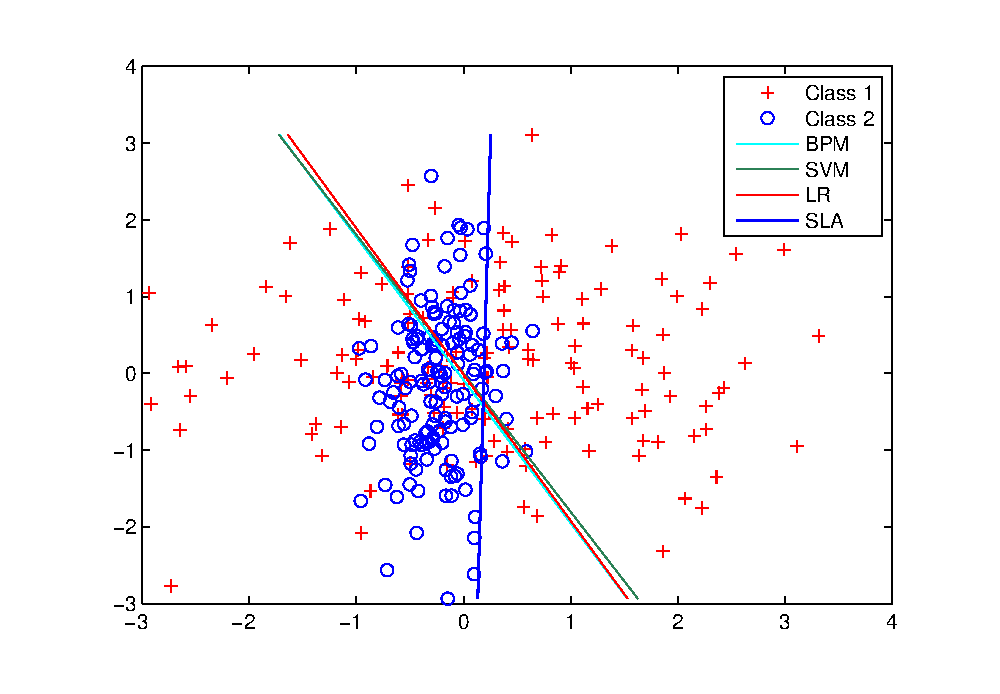
\includegraphics[width=0.50\textwidth]{images/fig63_633a.eps}
\caption{
This plot shows one example of a 2D anti-surrogate-loss dataset. Data points are generated in by two Gaussian distributions. In this case, BPM, SVM, LR give a similar 0--1 loss value around 120, which is 50\% higher than the optimal 0--1 loss value of 81 given by SLA.   
}
\label{fig:633a}
\end{figure}


\begin{table*}[htbp!]
\centering
\begin{tabular}{|cc|  ccc|c|}
\hline\hline
 && {\bf BPM} & {\bf SVM} & {\bf LR} & {\bf SLA}\\  
\hline
{\bf Best 0--1 Loss} && 
$120$ & $121$ & $121$ & $81$ \\  
{\bf Prediction Error} (\%) && 
$40.87 \pm 5.77$ & $40.16 \pm 5.84$ & $40.37 \pm 6.21$ & $31.88 \pm 5.95$ \\  
\hline\hline
\end{tabular}
\caption{Best 0--1 loss values and prediction error rates of each classifier for the anti-surrogate-loss dataset given in Figure \ref{fig:633a}.} 
\label{tab:antirates}
\end{table*}


Anti-surrogate-loss datasets occurred quite often during test data generation. These, however, have high dimensionality, hence are hard to visualize. Figure \ref{fig:633a} represents an anti-surrogate-loss dataset of $N=300$ found in 2D, where the best possible 0--1 loss value given by BPM, SVM, LR are 120, 121, 120, while the value given by SLA is 81, coincide with the minimum. Clearly, the 0--1 loss approximation accuracy of conventional algorithms is bad in this case, and this directly leads to poor result in the prediction accuracy test as follows. The test on the dataset given in Figure \ref{fig:633a} was performed using the same prediction accuracy testing procedure as stated in the previous subsection, however no noise is added. The results is shown in Table \ref{tab:antirates}. As can be seen, SLA error rate represents about 22\% improvement over that of existing algorithms. 

\begin{figure}[here]
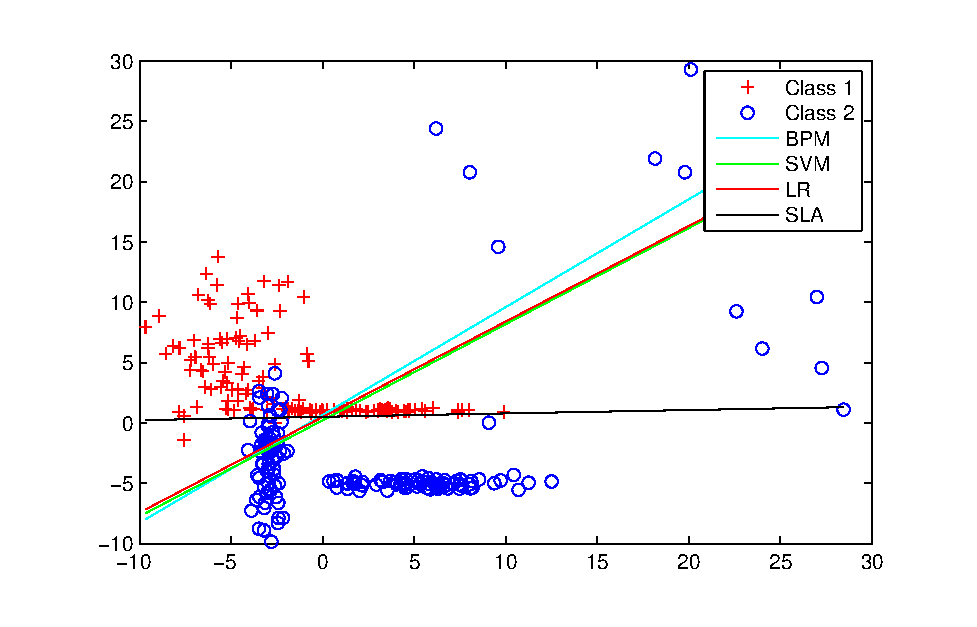
\includegraphics[width=0.50\textwidth]{images/fig63_633b.eps}
\caption{
Unlike the previous figure, this figure shows a dataset generated with 5 Gaussian distributions. In this case, existing algorithms give 0--1 loss around 74, while the value given by SLA is 26. 
}
\label{fig:633b}
\end{figure}

\begin{table*}[htbp!]
\centering
\begin{tabular}{|cc|  ccc|c|}
\hline\hline
 && {\bf BPM} & {\bf SVM} & {\bf LR} & {\bf SLA}\\  
\hline
{\bf Best 0--1 Loss} && 
$76$ & $74$ & $74$ & $26$ \\  
{\bf Prediction Error (\%)} && 
$25.66 \pm 5.33$ & $25.60 \pm 5.21$ & $24.27 \pm 4.83$ & $10.57 \pm 3.49$ \\  
\hline\hline
\end{tabular}
\caption{Prediction error rates and best 0--1 loss values by different algorithms for the second anti-surrogate-loss dataset given in Figure \ref{fig:633b}.} 
\label{tab:antirates2}
\end{table*}

Another (more extreme) example of anti-surrogate-loss dataset is given in Figure \ref{fig:633b}, where all commonly used methods give 0--1 loss values about 3 times higher than that by SLA. Comparing to the previous case, where data points were generated by two Gaussian distributions, the data points in this case were generated by five Gaussian distributions, hence confused conventional algorithms significantly. The result of the prediction accuracy test for this case is given in Table \ref{tab:antirates2}, where we see that the best prediction error rate among existing algorithms is $24.27\%$ about 2.4 times higher than the error rate of $10.57\%$ by SLA.

Yet another example of anti-surrogate-loss dataset was given at the beginning of the thesis in Figure \ref{fig:svm_failure}. In that case, conventional methods failed thank to the presence of outliers distributed in a specific region. In fact, it has been discussed very early in the thesis that algorithms based on surrogates of 0--1 loss are sensitive to outliers. 

May be there are more structures that make the dataset anti-surrogate-loss and the above are just to name but a few. However, the important message is that anti-surrogate-loss datasets are not rare, and in these cases, classifiers based on 0--1 loss, such as the proposed SLA classifier, give significantly better results than other classifiers based on surrogates of 0--1 loss.


%=================================================
\subsection{Summary}
\label{sec:rc.summary}

This chapter provided many tests and analyses to show the advantages and disadvantages of algorithms proposed in this thesis. It was verified that the result of PCS and BnB coincide with each other. Both these algorithms guarantee optimal solution at the cost of running time, so they are suitable for datasets of smaller size: $N \leq 200$ or low dimensionality $D \leq 5$. On the other hand, the two approximation algorithms provide solutions close to optimal at polynomial time. Among these two, SLA runs faster and produces similar result comparing to CSA. Thus, SLA is the preferred algorithm for large datasets.

It was shown by comparing with other commonly used and state-of-the-art methods, that the proposed algorithms, represented by SLA algorithm, outperform all existing algorithms in regards to 0--1 loss optimization, and classifiers based on 0--1 loss optimization offers lower error rate than other classifiers in the presence of noise and/or outliers. This difference is considerably magnified with anti-surrogate-loss datasets, where existing algorithms (BPM, SVM, LR) give poor results while SLA still performs well. 

